\section{\Large PROBLEM SET 2}
\subsection{Problem 2}

\subsubsection{Define orbit initial conditions and make sure you can propagate the orbit of the satellite over multiple orbits using either a Keplerian propagator or a numerical integration scheme.}

\subsubsection{In general the body axes are not the principal axes. Identify principal axes through the eigenvector/eigenvalue problem discussed in class and compute the rotation matrix from body to principal axes.}

To resolve an inertia tensor $\boldsymbol{I_{CM}}$ to a diagonal matrix of principal moments of inertia, there must exist a matrix, $\boldsymbol{A}$ such that the Equation \ref{eq:principal_moments} holds, where $\boldsymbol{I_{CM}'}$ is the principal moment of inertia tensor about the center of mass.

\begin{equation} \label{eq:principal_moments}
    \boldsymbol{I_{cm} A} = \boldsymbol{A I_{CM}'} 
\end{equation}

It can be seen that the principal moments of inertia are the eigenvalues of the inertia tensor and that the matrix $\boldsymbol{A}$ is a matrix whose columns are the right eigenvectors or the inertia tensor. For the AQUA spacecraft, the results that follow are shown below.

\begin{equation*}
    \boldsymbol{I_{CM}'} = \begin{bmatrix}
        17510 & 0 & 0 \\
        0 & 23616 & 0 \\
        0 & 0 & 36245
    \end{bmatrix} \text{kg} \cdot \text{m}^2
\end{equation*}

\begin{equation*}
    \boldsymbol{A} = \begin{bmatrix}
            0.0045  &  0.9949 &  -0.1011 \\
            -0.9986  & -0.0007  & -0.0520 \\
            -0.0518  &  0.1012  &  0.9935
    \end{bmatrix}
\end{equation*}

\subsubsection{At this stage you should have a simple 3D model of your spacecraft including geometry and mass properties of each element. This includes at least two coordinate systems, body and principal axes respectively, and the direction cosine matrix between them. Plot axes of triads in 3D superimposed to spacecraft 3D mode}

The body axes of the spacecraft are seen plotted in Figure \ref{fig:aquacad}. The principal inertia axes are seen plotted in Figure \ref{fig:aquacad_principal}.

\begin{figure}[H]
    \centering
    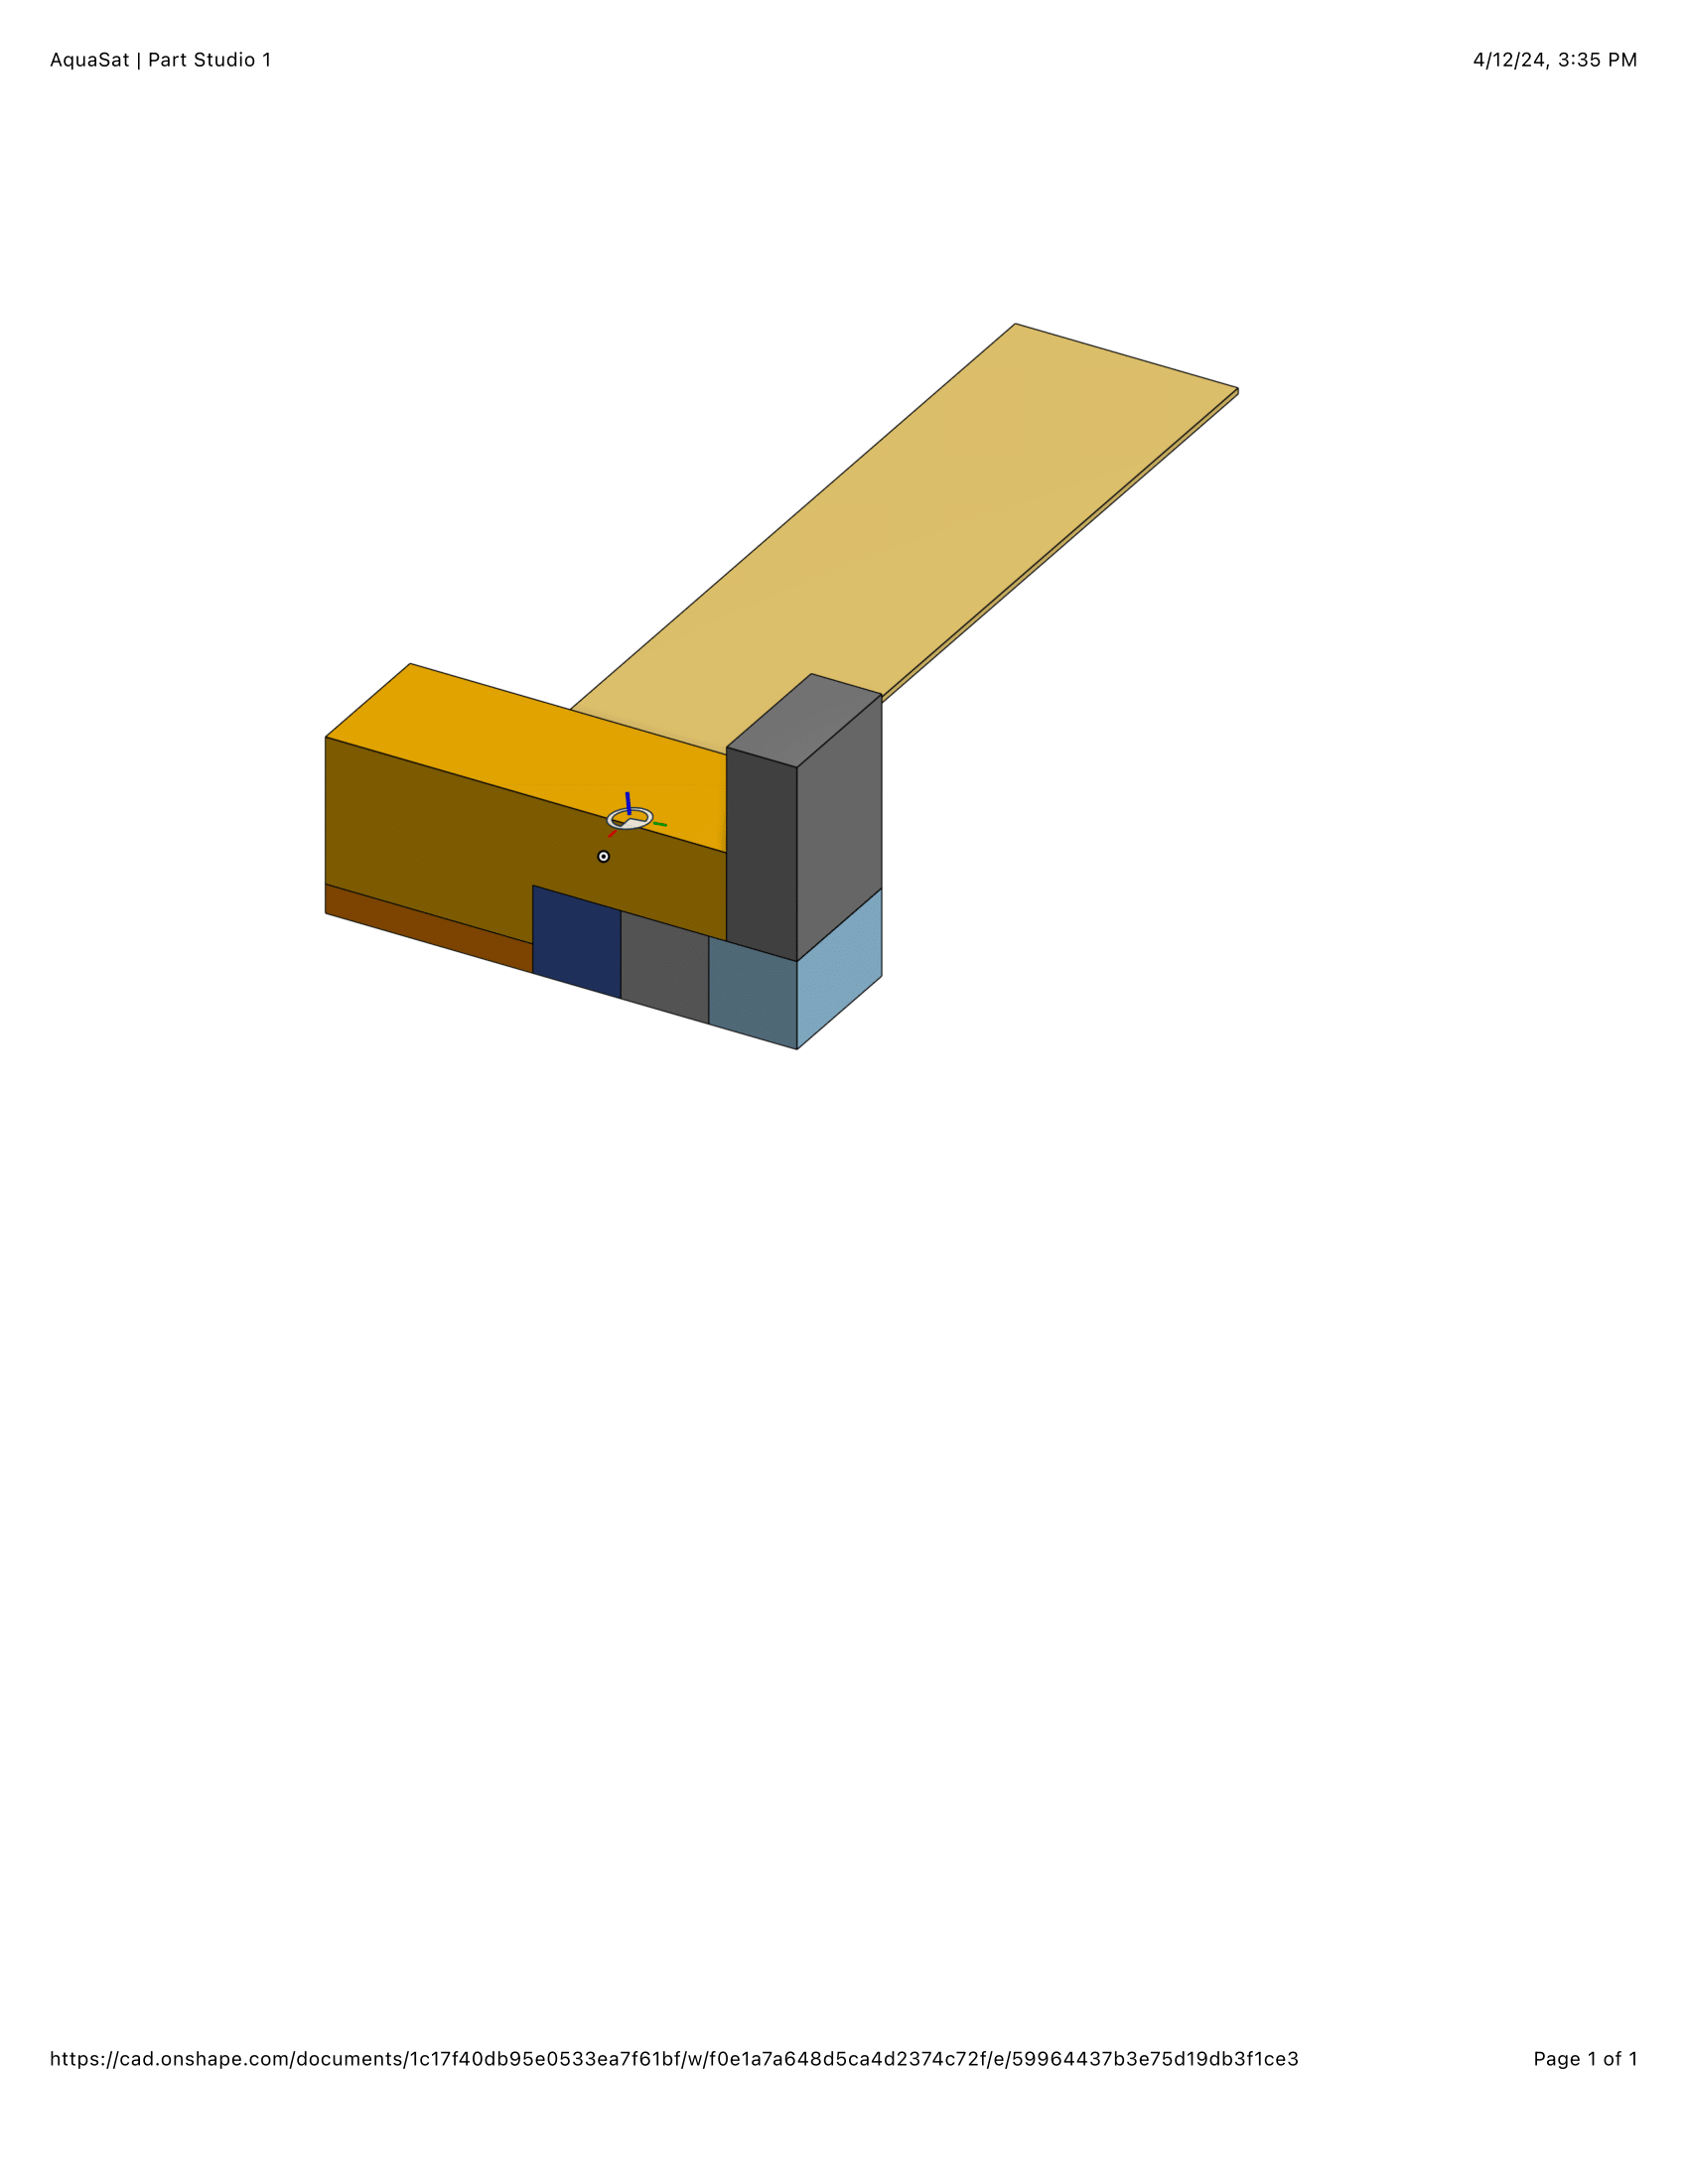
\includegraphics[width = 10cm]{Images/AquaSat_PrincipalAxes.png}
    \caption{Simplified Aqua Model with Principal Axes}
    \label{fig:aquacad_principal}
\end{figure}

\subsubsection{Program Euler equations in principal axes (e.g. in Matlab/Simulink). No external torques.}

\subsubsection{Numerically integrate Euler equations from arbitrary initial conditions ($\boldsymbol{\omega < 10^{\circ}/s}$, $\boldsymbol{\omega_i \neq 0}$). Multiple attitude revolutions.}

\subsubsection{Plot rotational kinetic energy and momentum ellipsoids in 3D (axis equal) corresponding to chosen initial conditions. Verify that semi-axis of ellipsoids corresponds to theoretical values}

\subsubsection{Plot polhode in same 3D plot. Verify that it is the intersection between the ellipsoid}

\subsubsection{Plot polhode in three 2D planes identified by principal axes (axis equal). Verify that shapes of resulting conic sections correspond to theory.}

\subsubsection{Repeat above steps changing initial conditions, e.g. setting angular velocity vector parallel to principal axis. Is the behavior according to expectations?}